\chapter{\label{5ethnographicField}Ethnographic Results 1: Culturally specific terrain}

\minitoc


\section{Abstract}
In this chapter I present the results of ethnographic data collected with the Beijing Men's Rugby team between September 2015 and August 2016.  I find a range of evidence in support of the predictions set out initially in Chapters 2 and refined in Chapter 3 in light of a review of the contextual specificities of the research setting.  First, I describe the culturally specific terrain of social cognition, which is defined by a dominance of ``hierarchical relationalism.''  The dominance of this culturally specific mode of social cognition is identifiable at multiple levels of social life, from the level of the institutions in which athletes, coaches, and officials interact, to the level of group norms in which athletes and coaches participate, to the level of on-field processes of joint action and perception.

                                          \begin{CJK}{UTF8}{gbsn}




\section{Analysis of Study Predictions: Culturally specific terrain}

In the ethnographic section of this dissertation, I make two sets of interrelated predictions.  The primary set of predictions derive from a novel theory of social bonding through joint action outlined in Chapter ~\ref{chap:theory}.  In addition to these primary predictions, I also predict that the specific group exercise setting of rugby in China will exhibit contextual specificity that will shape the contours of cognitive mechanisms and system dynamics of joint action and social bonding.  In this chapter, I report evidence for the second set of predictions of predictions---the culturally specific terrain of rugby in China---in order to lay the foundation for ethnographic evidence for the first set of predictions.

The culturally specific terrain relevant to rugby in China has formed through an ongoing interaction between the specific history of rugby and modern sport in China and facets of an indigenous Chinese psychology.  China is home to a dynamic indigenous psychology (see Chapter ~\ref{chap:researchSetting} Section ~\ref{sect:indigPsych}), which is the product of a number of distinct but interwoven historical trajectories.   Millennia of dynastic rule involving institutionalised norms of social interaction (commonly generalised as ``Confucianism'' or ``hierarchical relationism''), combined with draconian legal and bureaucratic mechanisms of governmentality.  At the same time, China represents to itself a narrative of rejuvenation as a modern Marxist/Leninist socialist nation-state, in the shadow of 150 years of colonial domination and humiliation at the hands of foreign (non-Han) actors (including Manchurian rulers of the Qing dynasty).  The project of modern competitive sport serves as a fascinating arena of social behaviour in which in which the dynamic interaction between, and interweaving of, these two cultural-historical trajectories is clearly choreographed.

Prevailing theory from the social cognition of joint action suggests that culturally specific terrain can function as informational affordances---``hyper-priors'' or ``coordination smoothers''---that functions to enable and constrain observable patterns of action, and perception, processes of group membership, and adherence to institutional norms \citep{Clark2015}.  Describing the terrain of the Beijing men's rugby team is thus an important first step to identifying ethnographic evidence for the hypothesised relationship between joint action, team click, and social bonding.

Conventional theories from within Western social psychology predict that social identity can be generated through a subjective process that is equivalent to calculating psychological distance between social categories of self and group \citep{Tajfel1971}.  As an extension of group identification theory \citep{Turner1987}, ``identity fusion '' represents extreme case that an individual perceives a 1:1 overlap between categories of self and group \citep{Swann2009}.  Related to these conceptions of social identification are theories of social motivation.  Motivation for pro-social pro-social behaviour, for example, is often conceived of as being inversely proportional to an individual's perceived distance between categories of self and group. 1:1 fusion between self and group entails maximal motivation to perform (potentially costly) pro-social activity on behalf of the group or individuals to which one identifies as fused \citep{Swann2015}.

In the case of China, however, social identity appears to be driven not by attention to perceived discrepancy between social categories of self and group, but more so by concerns for regulating and harmonising one's position within a network of hierarchically organised social relationships \citep{Liu2009}.  While distinct categorical modes of cognition related to the ``team'' and the institute are particularly salient in the context of the imported team sport of rugby, these categories do not appear to capture attention and perception in the same way as relational concerns.   In this Chapter, I argue, in line with existing research, that the distinctiveness of cultural terrain of professional rugby in China can be observed at multiple conceptual levels, spanning the social institutional level,  the level of group norms, and processes of (joint) action and perception.  I will offer observational evidence at each of these levels, before proceeding in the following chapter to an analysis of generalisable cognitive mechanisms of joint action and social bonding that are identifiable across and within this culturally specific terrain.


\subsubsection{Institution as platform for the social activity of hierarchical relational networks\label{sect:institutionPlatform}}

As explained in detail in Chapter ~\ref{chapt:researchSetting}, the Institute is one of four sports institutes in Beijing, and is home to seven sport programs.  One principal and four vice-principals overlook these seven sports, each principal being primarily responsible for one of the seven sports.  The Institute is of course held together by a bureaucratic backbone of rules and regulations that are decreed by city and central government.  These regulations set the parameters within which social interaction can take place.

Generally speaking, two key institutions are salient to athlete experience: the Institute (and the province or city that it represents, Beijing), and the rugby team itself.  Ethnographic observations reported herein suggest that while institutional categories are important platforms for social interaction, these two institutions do not play a dominant role in enabling and shaping social interaction and social identity formation.  Instead, concerns for regulating and managing hierarchically structured relational networks, particularly to one's own ``guanxi'' network, dominate attention and activity.  Institutions serve less as categories through which individuals calculate social identity, and more as a platform on which social activity of relational networks can unfold.

\myparagraph{Athlete motivations for rugby}
This conceptual distinction between institution as social identity category and institution as platform for social relationalism is observable in the way in which athletes report their motivations for playing rugby.  After I completed each semi-structured interview, I asked each of the 26 athletes to complete an activity in which they were asked to rank (from most important to least important) their motivations for adherence to rugby at the Institute.  I selected these motivations based on preliminary unstructured interviews and conversations with athletes, coaches, and other knowledgeable observers.  The motivations included: ``Education'', ``For Beijing'', ``Family'', ``Gain Respect of Others'', ``For Teammates'', ``Employment'', ``Beijing Residency'', ``Money'', ``Enjoyment'', ``Popularity (with prospective romantic partner).'' I wrote each motivation down on a piece of paper and scattered them randomly on the surface of a table in my room where I conducted interviews.

Results of this activity revealed the following mean rank of motivations:

  \begin{enumerate}
    \item Family (2.34)
    \item Education (2.38)
    \item To gain respect (from those around you)(3.50)
    \item To represent Beijing (3.58)
    \item Employment (3.96)
    \item Teammates (4.00)
    \item Enjoyment (5.69)
    \item Money (5.85)
    \item Beijing Residency (6.31)
    \item Popularity (with prospective romantic partner) (8)
  \end{enumerate}

It was telling to see that motivations of family and education ranked as the highest of athletes' motivations for rugby.  When asked in semi-structured interviews, almost all athletes agreed that their most prominent explicit motivation for playing rugby was to pursue life-course opportunities of education and employment.  Importantly, it was also commonly declared that achieving education and employment through commitment to rugby would make their families proud.  The fact that the opportunity for attaining tertiary education through rugby was more proximal to athletes than employment opportunities beyond university could perhaps explain the relatively lower average rank of employment. It was clear that most athletes were not immediately motivated by the promise of Beijing residency.  In sum, athletes' motivations for adherence to rugby indicate that concerns for life-course opportunities and family were on average more dominant than motivations driven by team-based categories such as ``For Beijing'' or ``For Teammates.''  As such, it is not the institution itself, but the social activity upon the platform of the institution to which athletes devote more attention.

Senior athlete Lu Peng provided a clear explanation for the prominence of education as a motivation for adherence to rugby:

\begin{quotation}
  Most of us in Shandong are like me, 80-90\% are of the same idea: there is an awareness that individual sports need less people, and so coming to rugby this type of team sport, most people’s goal is to use rugby to get to university.  But when I came to CAU I thought suddenly that I really like this sport, before I had never come into contact with a team sport before, and it was a team sport involving a ball, so I really liked it.
\end{quotation}

\begin{quotation}
  对,因为我们山东大部分人,都是像我这种,百分之八十到九十差不多都是这个思想,就是这么个意识就是说,单项需要人少,所以来橄榄球这类集体项目,大部分目的就是为了上个学。但是来到了农大之后我觉得我突然就喜欢这个项目,以前没接触过集体项目,而且有球的集体项目,所以我很喜欢。
\end{quotation}


During fieldwork I witnessed a number of instances in which an athlete's mood fluctuated according to the state of their attempts to secure life-course opportunities of education and employment.

Two senior athletes, Ma Haitao and Cui Suocheng, despite long qualifying as a Champion Athlete, were involved in complex bureaucratic journeys in an attempt to gain admission to BSU.  One day early in my first stint of training I was taking a training session in which we were focussing on defence, and Shuocheng suddenly appeared to have given up all energy.  He all of a sudden stopped doing the prescribed tackling drill.  I took him aside and began to take him through some of the details he missed last week when he was away.  He refused to listen and said, ``I get it, I just don’t want to do it, I’m sick of it, I’ve had enough of this drill'' (练够了!)''You’ve had enough?'' I asked, ``Alright, if you’ve had enough then get off the field!''  I snapped at him, motioning to the stands for him to go and sit down. I was stunned that he first said that he didn’t want to practice.  Shuocheng immediately followed my instruction and sat on a tackle bag on the side of the training field.  Later on in the training session, he came back over to the subsequent training drill and started offering advice to the more junior athletes about their technique.

A few days later I found an opportunity on our way back from training to the dormitory to ask head coach Zhu about the situation with Shuocheng.  Zhu explained that Shuocheng was experiencing difficulty finalising his contract transfer from Shandong to Beijing province, and that this procedure was interrupting his ability to process his university application (Shuocheng had moved from Shandong provincial team in 2014). To attain prized life-course opportunities through adherence to rugby was obviously a core motivation for most athletes.  But it is worthy mentioning how seriously these concerns appeared to grip athletes, to the extent that, in Shuocheng's case at least, his ability to train freely and openly was compromised.  Ma Haitao, another senior athlete also in the process of trying to apply for university (after years of delays), also experienced large amounts of stress during my time researching.  One day he spoke to me at length about the way in which these difficulties were impacting on his mood and his ability to focus on training. ``It impacts me so strongly'' he said as we walked to the canteen after a training session.  ``I’ll probably need to have a long sleep or take a break from training before I can recover from these sort of frustrations---the endless process of getting this form and completing that form, its so frustrating'' (CHINESE).

The fact that family was the highest ranked social category above team-related categories of ``For Beijing'' (4th) and ``For Teammates'' (6th) was indicative of the primacy of motivation related to immediate relational networks of each individual.  While representing Beijing was clearly important, and indeed rugby was the source of gaining respect from others (3rd), these motivations appeared to be coordinated by concerns primarily for family and life-course opportunities.  Very few athletes cited ``For Enjoyment'' (clear 7th) as the prime motivation for adherence to rugby.  It would not be inconceivable to see this as a strongly cited motivation for adherence to rugby in settings in which rugby exists as a popular mainstream sport.  Many, including some professional practitioners would claim to be adhering to a sport like rugby simply ``for the love of the game'' \citep{}.

\myparagraph{Individuals wield power, not the institution itself}
During my time conducting research at the Institute, I began to realise that individuals who occupied higher positions had considerable power to influence the social activity that unfolded in the institutions of the Institute and the rugby team within the Institute.   The head coach, for example, appeared to be very influential in deciding which athletes could participate in the team.  The change in head coach half way through my first stint of ethnographic research gave me the fortunate opportunity to witness the implications of this transition for the social organisation of the team.

When I returned to Beijing after a 10 day travel break in February, almost a month after head coach Wang had replaced former head coach Zhu, two of the athletes who were on trial under Zhu's tenure---XG and LJX---had since left.  When I asked senior athlete Wang Wei about the disappearance of these two students, he suggested that ``they had interests with Old Zhu...Old Zhu said that he could solve their ``school problems'' [i.e. get them into university]. They were here to try to get in to University.'' (和老朱有利益关系,老朱说可以解决上学的问题 都是过来上学的). Talk of arrangements of this nature in sport was hushed but common, and it came as no real surprise to me by that stage.

In fact, my question to Wang Wei that day was in part prompted by the fact that a group of four new trial athletes had just arrived from a high school in the neighbouring province of Hebei.  Apparently, someone in Wang's relational network had introduced these athletes to Wang, and they arrived at the Institute and joined in training for the day.  This coincidence was a telling indication of the power of the coach to coordinate the members and activities of the team.  The Institute and the team serve as platforms for activates of relational networks to unfold.  An athlete is only categorically related to the team by virtue of his or her capacity to adequately participate in and foster social relationships that play out on that institutional platform.  In this research setting, I found evidence that social categories of team and Institute served less as sanctimonious categories for social identity formation, and more as platforms for opportunity and advancement through regulation and harmonisation of relational networks.

\myparagraph{Leaders have the final say}
One striking example of the dominance of hierarchical relationism over categorical social identification as a director of social attention and action came towards the end of my second stint of ethnographic research. One week before the the final National Championship Tournament in July 2016 (the Tournament during which I performed the survey study (Chapter ~\ref{chap:trainingExperiment}), a very large and overweight young man appeared at training.  He did not appear to display any direct athletic potential relevant to rugby (he was quite heavy set and unagile), and it was also clear that he completely unfamiliar with rugby.  I was somewhat puzzled by this new arrival.

The only other analogous situation I had previously witnessed was occasional coming and going of the son of Vice-Principal Wang. Wang's son, known affectionately as ``Chubbsy'' (小胖), was a normal (non-athlete) student at a local Beijing high school student.  Chubbsy had no specific background in sport, but would join the team's training during sessions during periods in which his school was on holiday break.  Chubbsy had become a popular and welcomed presence in the team; he assumed the role of most junior member of the team and diligently performed all the tasks expected of him in this role (carrying training gear to training, filling water bottles, etc.). He had a positive and gregarious personality, and was willing to learn the many foreign and intimidating skills associated with rugby.
Indeed, over time Chubbsy became considerably less chubby, and more and more competent in rugby.

Originally I had not thought too much about Chubbsy's motivations for adherence to rugby during school holidays.  I assumed, perhaps somewhat naively in hindsight, that the Vice-Principal wanted his son to participate in a team sport which had many positive educational and health benefits.  I was forced to rethink this assumption once I discovered the reason for this newest arrival less than one week before the year's most important Tournament.  As coach Wang later explained to me, this young man was also a local Beijing high school student and was also related---in some more or less direct way---to a different Vice-Principal at the Institute (Wang didn't specify exactly who, apart from referring to them simply as a ``Leader'' (领导)). Wang explained that this student had arrived to quickly familiarise himself with rugby, because he was to be named in the Beijing team for the weekend's Tournament.  At some point during the Tournament, he was going to take the field, and in so doing, attain the athlete qualification standard of a ``Champion Athlete.''  This qualification would enable him to attend the prestigious BSU through the athlete pathway!

I considered this to be one of the most absurd events that I witnessed during my fieldwork.  The scenario chafed against all of my intuitions from a young age playing team sports and absorbing egalitarian and meritocratic cultural narratives common to Western democracies and particularly to my homeland of Australia---the land of the ``fair go'' and the ``tall poppy syndrome.''  A young, roughly 17 year old overweight student with no athletic ability and no familiarity with the game of rugby was planning (under the will and organisation of the those who wielded power in his relational network) to take one of the 12 positions available to the Beijing team and play his first (and probably only ever) game of rugby so that he could take the field and therefore receive an undeserved passage to a prestigious university.

``The Leader has the final say, I can't do anything about it'' (领导说的算,我没办法)said Wang, helplessly, when I pressed him on it.  Wang was only half way through his first year as head coach, and perhaps had been targeted as a coach who could be manipulated.  Indeed, it was quite possible that rugby more generally had been identified as a sport in which these types of activities were permissible.  Rugby, after all, was a cold gate sport of little standing in China---and this manoeuvre was unlikely to raise many eyebrows beyond those of the Australian anthropologist on the sidelines of an empty stadium at the National Tournament.  Clearly, this was an instance when the power enacted in the relational network was more dominant than the power of the social institution in which these hierarchically structured relationship were allowed to take place.  The categories of the team and the Institute held less sanctimony (if any), and the imperative of regulating and harmonising relationships in a hierarchical network demanded more attention.

Instances such as this one demonstrate that the relational mode of interacting captures attention and perception. Any sanctity around the institutional boundaries of the team or the Institute appears to be secondary to activity that appears on the surface to be purely strategic, but in reality stems from a deeply relational social logic to the research setting.



      \subsubsection{Social norms of group membership}

I also observed the dominance of a relational mode of social interaction when athletes were required to navigate processes of group membership tot he rugby program.  In the case of the Beijing men's team, it was not as if the category of team and egalitarian ``all-for-one, one-for-all'' overtures historically associated with the sport of rugby in particular were not present.  I would often observe senior athletes, coaches and officials deliberately drawing attention to the concepts of team and team commitment, particularly in team meetings.  Over time it became obvious, however, that the focal point of athletes' social attention was not the abstract notion of team membership as captured by the social category of the team, but rather the hierarchical system of relationships between team members and team leadership.

These ethnographic insights confirm theory from cultural psychology, which predicts that individuals from East Asian cultures will on average attend to the harmonisation of in-group relationships (over the cultivation of categories of social identity such as the self and in-group) as the core priority of social interaction \citep{Yuki2003,Nisbett2003}.  Beyond this level of prediction, however, there is very little empirical evidence within cultural psychology to suggest how East Asians and Westerners behave in group settings given these divergent modes of social cognition.  It could be predicted that Western subjects will on average be more likely to behave in ways that demonstrates dominant attention to social identity categories of self and group.  East Asian subjects, by contrast, will on average behave in ways that demonstrates dominant attention to the cultivation of a viable position within a network of hierarchical relationships.

As I explain below through reference to ethnographic examples, it is important not to conflate these two predictions as the inverse of each other.  When talking to people about my research I often encounter the folk-knowledge stereotype of East Asian social behaviour as involving self-less sacrifice for the benefit of the group; East Asians are very ``communal,'' etc.  These generalisations are problematic because they utilise resources that are more salient in Western modes of social cognition---i.e., categories of self and group---to theorise behavioural tendencies.  In fact, Cultural psychology does not make any explicit predictions about how the social categories of self and group feature in settings in which a relational mode of social cognition is dominant.

In this Section I present evidence that athletes utilise a range of resources to service attention to a relational mode of group membership.  Paradoxically from a Western standpoint, these resources include acts of self-promotion.  But when understood from the standpoint of an indigenous psychology in which social categories of self and group are secondary to relational processes, promotion of self does not challenge promotion of group, and in fact under certain circumstances can be understood as a viable strategy for the cultivation of relational harmony.



  \myparagraph{``I have become a social animal''}

During the course of semi-structured interviews, it soon became obvious that the concept of membership to an abstract category such as a sporting ``team'' was not indigenous to most athletes' experience before arriving at the Institute to play rugby.  17 of the 26 athletes included in the final analysis had transferred to rugby from other sports: 15 from athletics, one from football and one from basketball.  The remaining nine athletes had no specific background in sport before arriving at the Institute.  When I asked athletes what new things they had learnt from rugby, an overwhelming response was ``team awareness'' (团队意识).  For the majority of athletes who came from the individual sport of athletics (and the athletes with no prior team sport background), the team dimension of rugby was a distinctly novel experience, involving a suite of new social norms and requirements associated with group membership.

Guo Junping, the youngest and most recent of the arrivals to the program during my time conducting research, had very little to say during our interview. He did however comment enthusiastically on the novelty of ``team'': ``It was only when I started playing rugby that I knew what a team was, before when training for athletics (everyone) liked to do it on your own!'' (练的时候才知道团队,以前练田径的时候都喜欢自己一个人单干!) Lian Jianxiang, a young trialist at the Institute (the athlete who was relationally connected to Coach Zhu's, see Section ~\ref{sect:institutionPlatform}), went into more detail:

    \begin{quotation}
     Before I wasn’t used to it, and then later as began to interact with my senior teammates, I discovered that it was more or less the same as my previous (athletics) team, but just more cohesive.  But there was still a difference, for example in an individual sport you need to manage yourself and that's all, whereas team sports you need to consider more, you need to consider a lot of things that relate to everyone...[By now] I am used to it. I like this feeling [of team sport membership] more, its so much better than individual sport, in an individual sport its just yourself, its too independent. This (rugby) is a big family, isn’t it?
    \end{quotation}

    \begin{quotation}
      之前不适应,后来和师兄一接触发现和我之前的队也差不多,要团结。但还是有差别的比如说之前个人项目管好自己就行了,团体项目考虑的比较多,要考虑好多大家一起的东西...习惯了。更喜欢这个感觉,比个人好太多了,个人只不过自己,个人项目太独立了,这个是个大家么 \\
    \end{quotation}

  Unruly undergrad Fang Chao explains how he was transformed by rugby and the team:

      \begin{quotation}
        I think before when I was doing athletics, compared to now, I think I am a completely different person.  When I first came into contact with rugby, before I was doing an individual sport.  Now this is a team sport. I've changed a lot in terms of my personality, before when doing athletics I thought I was very independent and self-reliant, my own person.  Now I am one person who needs to communicate a lot with other people, cooperate; I have become a social animal.
      \end{quotation}

      \begin{quotation}
        我觉得之前练田径,跟现在橄榄球比,觉得我完全不是同一个人了。橄榄球刚开始接触的时候,之前田径是个人项目,现在是团队项目。性格方便改变很多,之前练田径是觉得我是个我行我素,自己一个人,现在我一个人还需要和别人多沟通,合作,变成群恤动物。
      \end{quotation}

Sun Hongwei's description of the team (reported in the introductory vignette to Chapter ~\ref{chap:theory}) offers a similar exposition of the novelty of the team dimension of rugby. As I explain in the following section, it appears that the team requirements of rugby were processed by athletes and coaches using social resources derived from an indigenous Chinese psychology.


\myparagraph{Team as family, teammates as brothers}
The concept of ``family'' was central to the rugby program's public discourses surrounding social norms of group membership.  From vice-principal Jenny, through to the head coaches, and the athletes themselves, family was the metaphor most commonly used to convey the requirements of each athlete in-group.  The metaphor of family contained room for expressing both the solidarity and emotional support of shared membership, as well as a justification for the hierarchical structure of the group.

Senior athlete Wang Wei offered his perspective on the family-like structure of the rugby program at the Institute:

  \begin{quotation}
    Its not as if there was not a lot of new stuff, because I guess at the time I was playing basketball---basketball is also a team sport.  But the only little bit that rugby made me experience was respect for elders, newcomers must respect senior team members, senior members must take care of junior team members, this is something that I didn’t experience in basketball.  At the time also I didn’t understand that much, I guess China has always had respect for elders, but it didn’t come up for me in basketball, and so then when I came to rugby my experience of it was very deep.
  \end{quotation}

  \begin{quotation}
     那倒没有很多,因为我当时打篮球嘛。篮球也是集体项目但是唯一一点和橄榄球比让我体会到就是长幼尊卑,新人得尊重老队员,老队员得关照小队员,这是我在篮球上面没体会过的。当时也没了解这么多,中国文化一直有尊老爱幼嘛,在篮球队没体现过,然后到橄榄球队还是体验特深的。
  \end{quotation}

Wang Wei first arrived at the Institute in 2011, during a time when the range in ages of athletes at the program would have been quite extreme, with the youngest athletes being around 16 years old, and the oldest athletes being in their mid 30s (the age range of athletes during my research was 15-28 years).  The conventions associated with family in China functioned as a resource that enabled Wang Wei to navigate the social terrain of group membership.

The prominence of conventions associated with family were identifiable in the naming conventions of the team.  As a general rule, when directly addressing elder athletes, an athlete would add the suffix ``\textit{ge}'' (哥) to the elder athlete's first or last name, to indicate that the elder athlete was relationally equivalent to an elder brother.  When addressing Han Xiaolong, the most senior athlete in the group, for example, athletes would commonly use \textit{Long Ge} (龙哥).  When referring to the coach, on the other hand, athletes would use either the formal and respectful ``Teacher'' (\textit{Laoshi} 老师), ``Coach'' (\textit{jiaolian} 教练), or the more colloquial suffix abbreviation of \textit{dao} (导). The naming conventions for the coach conventions for the coach derived from a Confucian tradition of master-apprentice relationships---originally structured on familial relationship conventions \citep{Spence1999}. When referring to a teammate in the third person, athletes would often refer to them as either their senior apprentice \textit{Shige} (师哥) or junior apprentice \textit{Shidi}(师弟), depending on whether the teammate was older or younger.  The network of relationships of the rugby team were thus modelled using hierarchical familial and Confucian master-apprentice relational conventions.

At the same time, the concept of ``team'' (\textit{tuandui} 团队) was also highly salient in group discourse. And indeed, as per the traditional discourses that frame rugby as a character-building team sport, ``team spirit'' (\textit{tuandui jingshen} 团队精神) and ``team work'' (\textit{tuandui peihe} 团队配合) were commonly invoked as ideal ethics of group membership for the rugby team.   Over time, however, it became clear to me that athletes' understanding of the concept of team was closely aligned with the more indigenous concept of family.

In an official team meeting approximately two months into my first stint of fieldwork, vice principal Jenny provided the most elegant and articulate example of discursively framing the group as a family.

    \begin{quotation}
      ...I very much welcome everyone to join the Institute's rugby team. I also hope that in study, living, and training, everyone will treat each other like their own siblings, with mutual tolerance and understanding.  I hope you are able to create a very good team atmosphere, and it is by no means easy, because everyone comes from all corners of the world. Everyone is an independent individual, more or less autonomous, prone to be relatively selfish, and may also have poor self-management skills.  But this all changes when everyone comes to this big family, because rugby is a team sport. In a team sport, everyone in the team needs to be twisted together into one single rope in order for that rope to send out a force. I don't wish to see cliques of twos and threes; or see you take the field with seven hearts, or with five hearts---rugby doesn't work like that. I wish that [when you take the field] everyone shares only one heart. Only in this way will our team be able to achieve good results.
    \end{quotation}

    \begin{quotation}
      ...非常欢迎大家加入橄榄球的队伍,也希望在以后学习生活训练过程中希望大家像亲兄弟姐妹一样,互相宽容互相帮助互相体谅,能够形容一个非常好的气氛,因为大家来自五湖四海,非常不容易。每个人都是独立的个体,多多少少都比较自主、比较自私、可能自我管理能力较差。来到这个大家庭之后,因为橄榄球是个团体的项目、团队的项目,需要大家队伍要拧成一股绳,发出一股力。我不希望大家三个一群两个一伙,上场之后七条心、五条心、不是这样。我只希望大家一条心。只有这样我们队伍才能打出好成绩。
    \end{quotation}

The concept of family offered dual affordances for processes of group membership.  On the one hand, the family represents a group in which every member contributes to and receives collective strength and support, by virtue of the solidarity achieved through group membership.  On the other hand, the family, and indeed, the team,  entails hierarchy.  In the formal setting of the team meeting, Jenny emphasised the former dimension of the family.  But it was clear from behaviours in less formal settings that the family also afforded attention to fostering hierarchy, whereby some individuals enjoyed privileged access to shared resources by virtue of their seniority.  The concept of team and its associated egalitarian ethics were, by contrast, insufficient as affordances for explicitly representing and navigating the dominant mode of hierarchical relationism.

\myparagraph{The coach is King...or Emperor?}
Over time I discovered that within the broader model of the team as family, certain relationships were highly valued and emphasised. It was clear that athletes payed special attention to their relationship to the coach.  Not considering the Institute leadership, the head coach sits clearly at the top of the apex of the team, followed by the senior athletes (Han and Lu - the old guard were also transitioning coaches), and then from there in order of seniority, which more or less co-varied with age.  When conducting the post-interview activities with Feng Yang, a young athlete who had been enticed away from the Shanghai team to Beijing by the promise of attending BSU, he asked me why I didn't have ``For Coach'' as one of the motivation categories for rugby:  ``Is there a Coach option in here?  I think there should be a Coach option!'' (这里没有教练吗?我觉得应该有个教练!)

Admittedly, I had not originally considered the Coach as a core category of athlete motivation, mainly because at the time I was not as attentive to the hierarchical structure of the group, and in particular the possibility that the coach would be singularly identified as a motivator of adherence to rugby (in distinction to the team more generally).  But the series of semi-structured interviews with athletes indeed demonstrated the centrality of the agency of coaches in their trajectories.

All athletes who had transitioned from a different sport previously (17) cited their previous coach as the agent of the transition: their coach introduced them to the Institute or facilitated a trial with the Institute, or directed them towards the opportunity.  It was clear that coaches were important figures in athletes' lives.  As explained in Section ~\ref{sect:institutionPlatform} above, the head coach of sporting programs is a key coordinator of opportunities and resources for athletes, and therefore it is understandable that the coach would be a central focus of social attention \citep{Yuki2005}.

As I became more aware of the prominence of the coach in the team hierarchy, I began to notice instances in which social norms concerning the coach were enacted.  I first began to notice the stature of head coach Zhu during meal times.  I noticed that Zhu and Shi had developed a habit of arriving at meals at least 15-20 minutes after all of the senior athletes who ate at the 1st Level canteen.  This timing meant that athletes were more or less finished eating by the time that Zhu and Shi had served their own meal from the buffet trays and prepared to sit down.  At this point, many of the senior athletes in the canteen would hastily finish their meals and leave the table before Zhu and Shi arrived (each sport program at the Institute was assigned a set number of circular tables at which to sit and eat, thus the coaches invariably ate with the athletes). At the sight of Zhu and Shi entering the canteen, some of the athletes, commonly Wei Wenxin and Wang Wei, would quietly cry out under their breaths something like ``Quick, Old Zhu is coming!  Let's go let's go!'' (快点,老朱来了,走吧走吧!) and attempt to leave without having to interact with the coaches.  I noticed that members of the Old Guard, particularly Han and Lu (who were technically speaking coaches themselves) often ignored the urgency of departing before the coaches arrived, and would stay and keep the coaches company. Other times, if they had well and truly finished their meals or had somewhere else to be, they would join the other senior athletes in escaping and clearing their trays in the canteen's kitchen.

I later asked Han why athletes were so keen to escape, and he suggested that if they were still present at the table when Zhu and Shi arrived to eat, then they would feel strong social obligation to accompany the coaches through the full course of their meal, and only leave once the coaches had finished eating.  On some occasions, the Zhu and Shi would arrive slightly earlier, before some athletes were able to finish their own meals.  In these instances, I noticed a combination of strategies, all of which involved seeking permission or receiving permission from Zhu to leave the table.  Zhu would often notice when athletes were finished their meals and would actively grant permission to the athletes: ``If you've finished eating you can go''(吃完了可以走吧).  Often athletes would wait for this permission rather than asking for it themselves.  Han explained to me that Zhu and Shi had deliberately developed a habit of arriving late to meals so as to reduce the frequency of scenarios in which this social tension arose.  It was clear that both parties perhaps wished not to have to engage in this social ritual of respect to authority of the coach, but were unable to escape participation in the social convention when the appropriate situation arose.

I soon discovered that I was also afforded this treatment as a coach, although I could tell that because I didn't feature as centrally in the orbit of relations in the same way as the head coach, the social charge of my presence in these situations was much less intense.  Athletes were happier to freely announce to me that they had finished, and I awkwardly insisted that they leave.  When Wang became head coach, the tension in these situations was drastically reduced. Wang after all had himself been an athlete and played alongside many of the athletes who he was now eating with.  He usually chose to arrive at around the same time as the other athletes.  Even though athletes were more comfortable with Wang than with Zhu, they still had to enact the ritual of asking for leave if they had finished before Wang.  This convention around meals is indicative of the importance of particularistic hierarchical relations in structuring social attention of group members \citep{Liu2009}.

\myparagraph{The ``I'' in team}
The clear social authority of the coach over athletes is understandable in the context of an indigenous Chinese psychology containing elements of Confucian values of hierarchical relationalism.
Available evidence in cultural psychology and my own surface-level assumptions about Chinese indigenous psychology did not prepare me to interpret what I saw as instances of self-promotion in group contexts.  These behaviours appeared odd to me, given my egalitarian impulses: the promotion of the individual as the primary agent seemed to create tension between category of self and group, whereby the importance and sanctity of the group category was de-emphasised.

I started to notice this in interviews when I would ask about each athletes' journey to rugby.  Although athletes would recognise in passing the agency of their coach or close relation who facilitated their journey to the Institute, when I asked whose final decision it was to play rugby, almost all athletes would emphasise that coming to the Institute was ultimately their own personal decision.  Often this personal agency was made in distinction to their parent's will.  Senior athlete, Ma Haitao, after explaining how he had been introduced to rugby via one of his family friends (who had attended CAU), explained how he came to the decision to play rugby:

  \begin{quotation}
    My Father didn't know this sport.  Because in China very rarely will people know what this (rugby) is, so my Parents didn't know. From a young age I've been away from home doing sport, and so generally I decide these things...I made the decision myself.  At the time I arrived wheeling a suitcase and had a bag on my back.  I came at the time with a classmate...
  \end{quotation}

  \begin{quotation}
    我爸不知道这个项目。因为中国很少知道有这个,他们不知道。我从小就在外面练体育,所以我一般是自己决定这些东西\textellipsis自己决定的。当时自己背个包投的箱子来。当时和一个同学,他是农大的。
  \end{quotation}

Meng Cheng, a junior aspiring athlete from Beijing's outer suburbs was even more proud that the decision to play rugby was his own:

  \begin{quotation}
    My parents at the time thought [rugby] was quite dangerous, and they didn't let me play.  But they weren't as stubborn as I was.  It's the case with everything, I decide...If I to do something I have to make the decision myself, and then no one can change my decision\textellipsis
  \end{quotation}

  \begin{quotation}
    父母当时觉得很危险,不让我练。但是拗不过我,他什么事都。我自己决定了\textellipsis
    就是说我拿什么我一定拿的主意,任何人改变不了\textellipsis
  \end{quotation}


  Pan Qiyu, a senior athlete and CAU graduate from Dandong in Liaoning province, also had a similar story about self-determination when I asked him about his decision to play rugby:

    \begin{quotation}
      I decided myself\textellipsis How I came to the decision was actually quite interesting.  At the time when we first came in it was really difficult.  At the time forty or more of us were selected, but many people wouldn't let us train, including our head teacher at high school.  A lot of class teachers said to me that there was no hope for rugby, rugby in China has no development [potential], and there are barely any universities that you can attend [through their rugby programs].  And so then they wouldn't let us (the students who selected rugby) train, only us! After that I said to my Mum and Dad that I really liked this sport, and then my parents also extremely supported me with this.  When I got in to CAU (through their rugby program) my parents were extremely supportive.
    \end{quotation}

    \begin{quotation}
      我自己做的决定\textellipsis决定特别有意思。当时我们进来的时候特别艰难,当时我们选了四十多个人,好多人不让我们练,包括我们的班主任,好多授课老师跟我说没什么希望,橄榄球在中国没有什么发展, 也没有几所大学能上。然后不让我们练,就——我们! 后来我就跟我爸妈说我特别喜欢这个项目,然后我爸妈也非常支持我,我靠农大的时候他们非常支持我。
    \end{quotation}


The pattern of athletes emphasising their own determination in the decision to play rugby was striking, particularly when combined with the fact that almost all athletes also mentioned---more incidentally and as matter-of-fact---that their coaches played some sort of role in facilitating the opportunity to play rugby.  In other words, it was unlikely that these individuals were the sole determiners of the decision.  It was clear that there was some social utility to emphasising self-determination, as if it was an important virtue of group membership.

%johnnyZhangKids
The virtue of self-determination and self-reliance was powerfully illustrated to me outside the context of the Institute, when I agreed to help out CAU coach (and China's most famous rugby player Johnny Zhang) by agreeing to take a rugby session with a group of young school children (aged between six and eight years).  The training session was designed to be explicitly educational, and so I felt that I should attempt to tie some of the elements of team work in rugby to virtues of friendship (see Figure ~\ref{fig:johnnyZhangKids}).

Towards the end of the session, when trying to emphasise the importance of teamwork in a team relay drill, I asked the children: ``Who do you rely on most in this life?'' (你在生活中最依赖谁?).  I was hoping that this question would naturally prompt the answer that they had to rely most on their family and friends for support---what I thought was a relatively obvious response in either a Confucian or Anglo-Protestant system of ethics!).  To my surprise, a chorus of two or three more outspoken children responded, instead: ``Myself!'' (自己!) We rely most in life on the self, these kids insisted. Self-reliance was not the reply I was looking for, but it did say something about the emphasis on self-reliance as an important virtue of group membership.  Indeed, consultation of Chinese indigenous psychology reveals that self-cultivation is a central virtue in a Confucian system of ethics, and is a central resource necessary to foster viable social relationships \citep{Liu2014}.


\begin{figure}[htbp]
  \begin{center}
    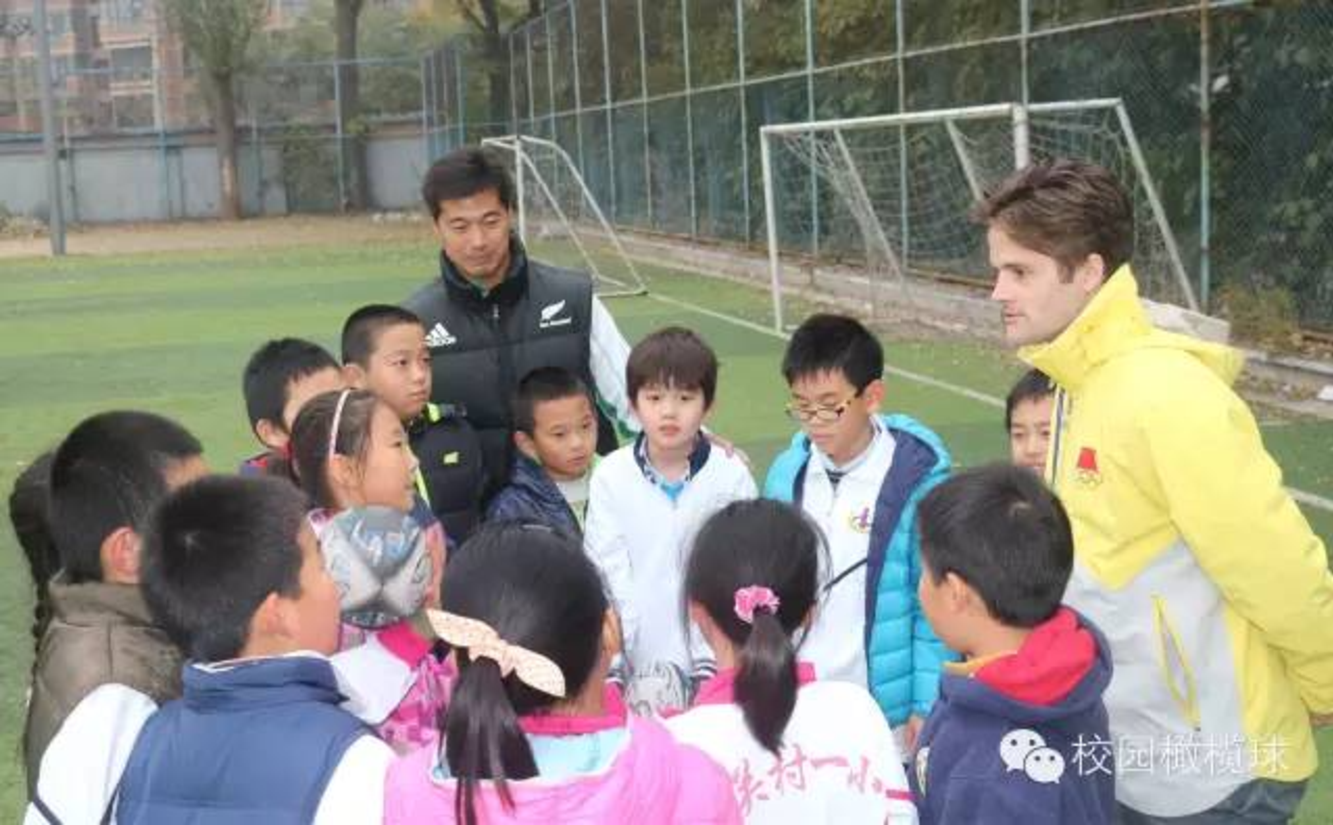
\includegraphics[scale=.6]{images/johnnyZhangKids.png}
    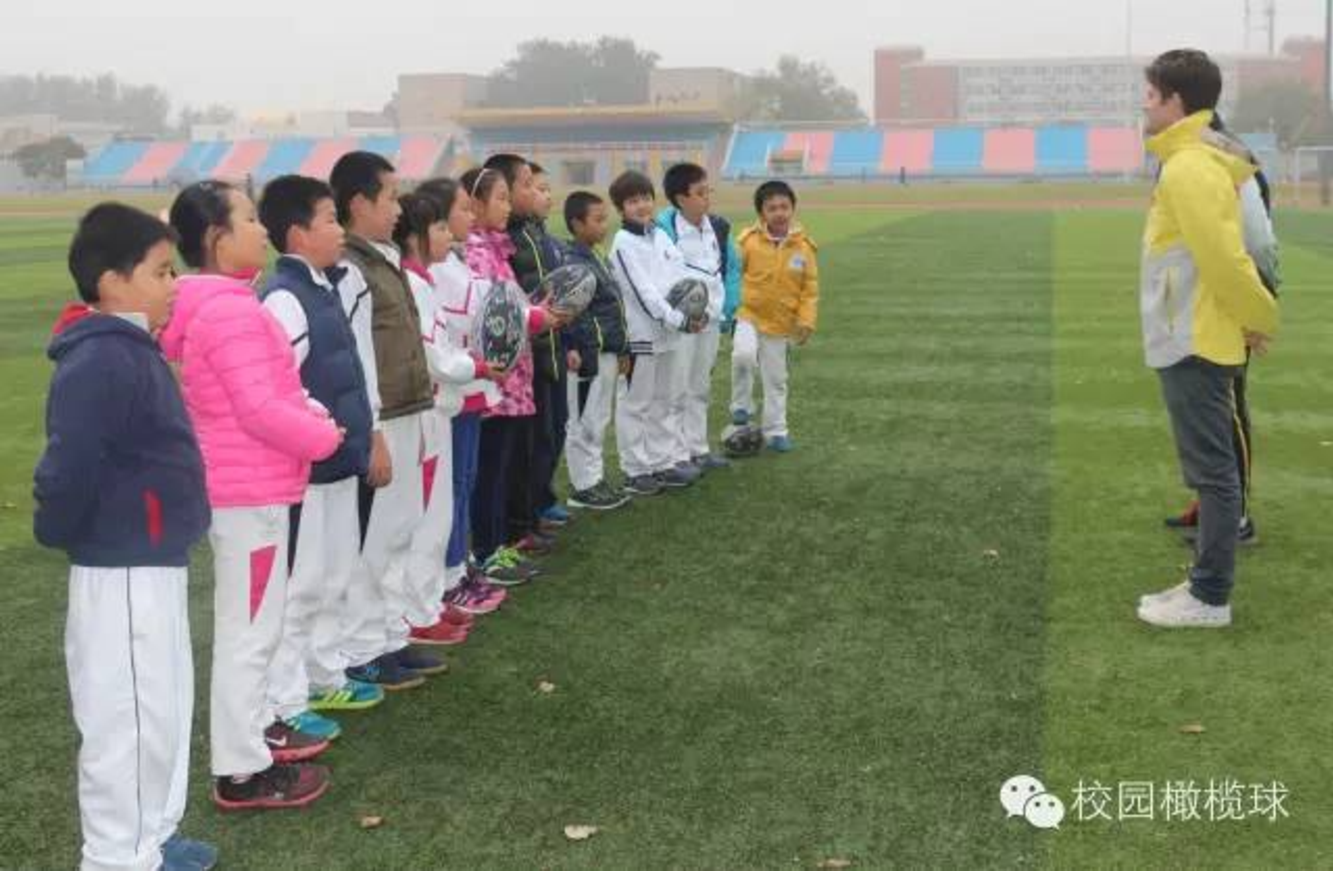
\includegraphics[scale=.6]{images/johnnyZhangKids1.png}
      \caption{Me taking a training session with a class of Chinese kids CAU coach Johnny Zhang}
        \label{fig:johnnyZhangKids}
   \end{center}
\end{figure}


The active cultivation of the self was a recurrent theme in interviews with athletes when asking about their role in the team and how they ought best contribute to the team.  As unruly undergrad Hou Siqi explained when I asked him if he considered his teammates as an important part of his motivations for adherence to rugby:

\begin{quotation}
  I think about them (teammates) little bit, but I think after all the main thing is to make sure you do a good job your self.  When you're looking after your self that can be a foundation on which to consider others.
\end{quotation}

\begin{quotation}
  有一点,但是我觉得我毕竟是主要还是想把自己做好,做好自己的基础上为再考虑大家.
\end{quotation}

When I asked another unruly undergrad, Fang Chao, about his perceived role in the team, and what he ought to focus on, he responded that he ``hadn't thought that much about it, I just want to make sure I play well myself, ensure that I personally train hard'' (我没想那么多,就想自己把球打好,自己好好练).

%\subparagraph{Captain Han's speech at the team dinner}
The importance of self-assertion and promotion within the context of the team was performed at a team dinner held on a Sunday night (when everyone had returned from leave) a few weeks after Wang took the reigns as head coach.  This team dinner, like the team dinners that I had previously attended, was held at a Shandong restaurant a 10 minute walk south-west of the Institute's Main Gate.  It was the first team ritual orchestrated by Wang, and as such Wang initiated a ceremony of organised drinking and speeches.  I entered late and noticed that many of the junior athletes appeared nervous and up-tight. Almost 26 athletes were crowded around a large (but not that large) banquet table.  Wang sat in the position opposite the entrance to the private dining room (the equivalent of the ``head'' of the circular table).  Either side of Wang sat Han and Lu (the assistant coaches) and then the senior athletes in order of seniority, all the way until the opposite side of the table, where the most junior athletes were positioned.

Wang began the proceedings with three toasts (customary as the host), and then from there the senior athletes spoke in turn.  After each toast, the entire team had to drink a portion of their rice wine (and then beer after the rice wine had been drunk).  After the senior athletes had all had a chance to talk, the coaches directed each vague cohort of athletes (i.e., the very youngest athlete on trial, the aspiring Chaoyang students, the unruly undergraduates, and then the remaining senior team) to stand up and say a few sentences and then drink to the coaching staff (and senior athletes).

The proceedings were relatively rigid to begin with, and from my position to the side of the table, the scene resembled an awkward face-off between the senior athletes and coaches at one end of the table, and junior athletes on the other end.  But once the alcohol kicked in, social interaction began to flourish. Speeches became bold and fluid with both self-assertive pronouncements and self-critical admissions, and the spaces between formal toasts were filled with one-on-one sideline conversations between athletes and coaches, junior and senior intermingled.

Han's first speech, which came after Wang's three toasts, was one of the most bold and noteworthy:

  \begin{quotation}
    I don’t know if all of you have your own personal goal?  I at least know that I have a goal, and that is to win next year’s National Games gold medal.  That is what motivates me; that is what I am sacrificing for.  I don’t know exactly what your goals are, but if you don't have a goal then your (personal) goal should be to help me achieve my goal.  I toast to everyone helping me achieve my dream of winning a National Games gold medal!
  \end{quotation}

  \begin{quotation}
      我不知道你们都有自己的目标吗? 我至少知道我有一个目标,那就是拿到明年全运会的金牌。 这就是我的动力,就是我所牺牲的。 我不确定你的目标是什么,但如果你没有目标,那你的目标应该是帮助我实现我的目标。 我向所有人致敬,帮助我实现自己的梦想(赢得全国运动会金牌!
  \end{quotation}

I was once again automatically struck by this bold speech.  Han was the most senior athlete in the team, he was the former team captain and was now in transition to coach.  I suspect that the intuitions around team membership that I had generated in rugby contexts elsewhere prepared me for a speech in which Han would take responsibility for curating an egalitarian idea of group membership.  ``We are all equal under the category of the team,'' he ought to say; we are all in this together.   Instead, in his prime-time team captain talk, Han was intuitively compelled to demonstrate the strength of his own personal conviction in order to generate solidarity. Han's speech appeared to me on the surface of things to be deeply self-promotional act (at the expense of an egalitarian ethic of equal access to the resources of team membership). But on another level, Han's speech could be interpreted as being deeply prosocial, as it expressed the strength of his motivation as a leader of the team. On this level, Han's speech expressed that he was upholding his part in the system of hierarchically structured relationship that made up the Beijing men's rugby team.  In this way, Han's dream was the group's dream, and Han's prosociality needed not be mediated through reference to the category of team and an egalitarian membership to that category.

Later in the evening, as the speeches progressed around the table, I did hear some of the more junior senior players make reference to team ideals.   CAU graduate Pan Qiyu suggested in his speech that ``we all need to put ourselves after the team; this is a team sport'' (我们都有把自己放在团队之下); and old head Wang Wei: ``this is a team sport; team first, self second'' (这是个团队项目。团队第一,自己第二)。 Importantly, however, these assertions were not egalitarian in their essence, and instead suggested an individual subservience to the team, rather than an egalitarian, shared ownership of the team by each of its members (a more common notion expressed in Western team sport contexts that I have been a part of previously).  Indeed, when Pan and Wang were referring to the team, it could be assumed that what they had in mind was a relational network of individuals structured in a fashion that mirrored the seating arrangement. On one level, the team was united together as equals: all of its members sat at a round table in which everyone had a seat. But on another level this circle was imbued with a hierarchical structure through which relations of power that flowed from the coach at one end to the most tenuous and junior athlete sat nervously awaiting orders at the other end.

While these two levels of social interaction could conceivably be identified as mutually co-occurring in equivalent settings across human cultures and throughout time, it is important to notice that this specific cultural milieu preferenced attention to the second, relational level as the dominant mode of social activity.  On this relational level of social interaction, categories of ``team'' and notions of team membership were present and salient in social discourse, but these categories appeared to function not as direct mechanisms for psychologically mooring individual identity to group identity (as social identity theory would have it), but instead as resources for reproducing a hierarchical network of relationships in which each individual was defined and visible only in his or her relations to others in that network \cite{Yuki2003}.



\myparagraph{The entire system must be aligned}
I encountered a number of instances in which it appeared that athletes' perceived their social domain to extended well beyond the interplay of immediate categories of self and the group.  Instead, categories of identification were porous, and what was essential was an element of coordination or alignment between elements. I outline a collection of examples below, and explain how I see these instances as evidence of the fact that social attention is directly predominantly towards management of hierarchical relationalism.

One example occurred the first morning I arrived back for the second major stint of ethnography in the summer of 2016. I arrived back to a terrible incident in which some of the rugby team had been effectively poisoned accidentally by pesticide sprayed on the hedges outside their dormitory windows.  A few days before I arrived back, the groundskeepers had carelessly sprayed pesticide on the hedges outside the windows of the bottom-floor dormitory rooms of which the rugby team were inhabitants.  Some of the pesticide had made it in to the rooms of the athletes via open windows, and had caused a few of the athletes to develop throat irritations and coughs.  Wei Wenxin, who replaced Han Xiaolong as team captain after Han was promoted to assistant coach, was one of the most seriously affected by the pesticide, and when I sat down with him at breakfast the first day I returned, he explained the story with deep anger and outrage.  Importantly, when I asked him what was going to happen with all of this, he said to me ``the Leadership will have to say something about this, we are all waiting to see how Leadership will respond.'' (领导们必须要说话,我们在看领导们怎么说). I found it interesting that Wei was so emphatic about the primary role Leadership ought to play in adjudicating this matter.  The role of political leadership in an organisation such as the Institute was no doubt crucially important to manage such issues, but the fact that Wei was so emotional and emphatic about this fact---almost as if the Leadership had a paternal role to play---was revealing of the emphasis Wei placed on an the need for alignment between levels of the social system in which he was situated.

Also during my second extended period of ethnographic research, which was well into the transition from head coach Zhu to head coach Wang, I shared a dormitory room with head Coach Wang's offsider, assistant coach Zhu Jing.  Zhu Jing had recently arrived from the rugby program at Xingjiang province, after Wang invited Zhu to join him as assistant coach.   Wang needed Zhu for support: to be his loyal leftenant, and to lighten the load on player-coaches Han and Lu. Despite transitioning to the official position of coach, Han and Lu were still required to train and play, at least until the National Games in 2017.

Zhu Jing was a new arrival to the team, and was thus on unstable ground. At the time he had no official contractual relationship with the Institute, and his position was therefore tenuous and contingent on his relationship with head coach Wang.  Zhu was neither a particularly celebrated rugby player during his time as an athlete at CAU, nor was he a particularly experienced or successful coach.  What he did posses, however, was a close relationship to Wang (they were classmates at CAU). Zhu was valuable to Wang for his loyalty---useful to Wang in his attempt to stabilise his leadership of the team---an inherently slippery platform for social activity (see Section ~\ref{}). In terms of his value to the team as a rugby coach and the Institute, however, Zhu still had much to prove.  If I were in his position, I thought, I would have done everything possible to help head coach Wang and the Team to improve performance.  As part of this, no doubt, I would seek to signal diligence and commitment in the way I went about my business as a coach.

After about two or three weeks into our roommate relationship, it became clear to me that Zhu Jing was not so concerned with signalling diligence, at least not to me, and not to the athletes either, at least not in a way that I recognised.  Most mornings I would wake up at 0700 to attend breakfast with the athletes and then collate my field notes and prepare for morning training, starting at 0900. Zhu, on the other hand, would reliably sleep through until roughly 0850 each morning, and then turn up to training usually at around 0920 after athletes had completed their warm up.  After lunch, Zhu would return to bed, usually from 1300 until 1500-1530, depending on when afternoon training was scheduled.  Afternoon siestas are admittedly an institutional part of China's work life, but routine indulgence in a two-hour nap was surely taking the institution to its extreme.  I rarely witnessed Zhu spend any time working on preparing training schedules or other forms of professional development.  As it turned out, head coach Wang also began to notice the way in which Zhu was approaching to his job.

After the final Tournament in Qian An in July 2016, the team went out together for dinner.  This dinner was much less ritualised than the first team dinner organised by Wang earlier that year.  This time,  junior athletes were in one room, and the senior athletes and coaches were in another room, free to socialise within their more naturally occurring social factions.  Towards the end of the evening, after the effects of alcohol had well and truly set in, a heated discussion developed between head coach Wang and assistant coach Zhu. The discussion began with one of Wang's numerous toasts to the group at the table.  Wang said that it was important that the rugby program distinguished itself as an excellent team at the Institute, and there was a need for all senior members of the team (seated at the table) to contribute to this project.  It became clear that Wang wished to emphasise the need for Zhu in particular to ``lift his game'' in this regard. Wang explained that as head coach he was burdened with a lot of administrative work that detracted from his ability to manage athletes and training.  Given that the team was without a dedicated team manager (who would usually manage daily concerns of athletes and organise team logistics), Wang suggested that Zhu ought to improve his contribution. ``As an assistant coach, you need to conduct yourself at a high standard'' (当助理教练你要作为一个高度) said Wang directly to Zhu, indicating that his current standard was not acceptable. Wang spoke politely, but the public nature of these remarks suggested that he was using the opportunity to criticse Zhu.

Zhu retorted defiantly, directing attention away from his personal standards to the global situation of the team at the Institute.  Zhu suggested that the most important thing was that the leadership of the program supported the program, and only then could the program achieve a high standard: ``you have to have the support of leadership'' (必须有领导的支持).  Lu and Han, the next most senior team members present, also became involved in the discussion, with Lu siding more with Zhu and Han siding more with Wang.

The next morning, Zhu and I lay in our dormitory room beds hung-over after the team dinner the night before.  Zhu revived the dinner incident with me, seeking my support for his position.  Zhu insisted that his ability as an individual was fundamentally limited if the Leadership did not appear to offer him support.  Initially I was in no state to record or write down Zhu's remarks, but his message was clear. If the team does not have the faith and support from the Institute (which in this case, it clearly did not have, at least since 2013), then how was Zhu supposed to perform his role?   I could see the point he was making, but the combination of my own deep-seated intuitions about ethics of group membership and self-conduct an unstable stomach, meant that I couldn't help but challenge Zhu on his line of reasoning.

After all, I thought that the clear way to counteract lack of support from the powers above was to demonstrate self-competence, to signal diligence and willingness to move independently, despite or in spite of the level of support form leadership.  As I looked at the state of the team, there were clear problems that needed addressing by someone like Zhu.  There was an apparent lack of clean and clear team discipline, a lack of focus, intensity, and technical precision during training, a lack of physical fitness necessary to survive the challenges of a high level rugby tournament, and so on.  These were all things within Zhu's remit, and that hard work from Zhu would help to address, I thought.  In this ``chicken and egg'' scenario that Zhu had generated via his defiant response, I thought that the team was a chicken with the capacity to independently lay an egg that would change the Institute's view of the rugby program, from the bottom up.

But Zhu pushed back.  He had experienced this situation before with Xinjiang Province during the last National Games.  The Leadership started off being very positive about rugby, promising this and that, but then in the end, nothing came through.  The support of leadership is hugely important in China: money, incentives, all of it.  If you don't have support from Leadership then you can't get anywhere.  Zhu was obviously defensive about the situation, attempting to deflect any blame or responsibility for his action (or lack thereof).

But perhaps his claims weren't completely unreasonable in the specific environment---an environment in which hierarchical relationism was a dominant mode of social attention.  In a way, Zhu was referring to the importance of the harmony of the whole system of social relations in which he was embedded as but one node situated at but one level. Individuals can only act with agency if the relationships that they attend to also sanction that agency, Zhu was effectively suggesting.  In the hierarchical system of relationships at the Institute, the crucial node in the system is the paternal benevolence of Leadership.  In this dominant paradigm, social institutions of self, team, and institute do not provide resources for agency and action in and of themselves, and rather act as platforms for the fostering of particularistic relationships in which agency is located.  In this way, Zhu's stance mirrored the explanation I had received from Wei Wenxin a few weeks earlier, the morning I first arrived back to the Institute for my second stint of ethnography: ``We are all waiting to see how Leadership will respond.''


\myparagraph{``Its all very complicated (in China)''}

Various instances during fieldwork gave me the impression that individuals employed a working mental model of the hierarchical network of social relationships within their social orbit.  Many of the athletes and coaches with whom I would informally converse would insist to me that China's social interactions were ``too complex'' (中国社会太复杂了), to a degree that I---a Western/outside observer---would struggle to fathom. I didn't grasp the depth of meaning of this at the time, and I simply assumed that my interlocutors were using ``complexity'' as a convenient word to account for the complicated gulf in cultural understanding between East and West.  While this reading is likely accurate on one level, after hearing this statement over and over again in response to my various inquisitions, I came to realise that my interlocutors' use of complexity may relate to the way in which sociality is concveived and represented in China.  In particular, complexity offers a way of capturing the attention that each individual is required---by deep-seated cultural convention---to to devote to fostering and harmonising an hierarchical network of relations in which the individual is understood to be a single node rather than an autonomous, bounded entity.

One day at breakfast, for example, Han started dreaming:

\begin{quotation}
  It would be great to live in the West, wouldn’t it Li Jie?  An hour’s work is an hour’s pay.  Not like China.  What’s it like it in China? ``You’re mine! (says your boss) You have to do whatever I say.''
\end{quotation}

\begin{quotation}
  在西方生活多好,多吧,李杰?一份货是一分钱。中国就不是了。中国是什么呢?你就是我的人! 你要听我的!
\end{quotation}

Clear in Han's dreaming was a representation of the social regime in which he imagined he was positioned---one of interdependence within a hierarchical network of relationships.  The act of comparing China and ``overseas'' (\textit{guowai} 国外) or ``the West'' (\textit{xifang} 西方) became a common theme when I would discuss issues with predominantly senior athletes and coaches.

%Question of belief
``Long live Chairman Mao!'' (毛主席万岁!)I said jokingly one day during my first stint of ethnography as I caught up to the group of senior athletes headed to the canteen for lunch.  ``Long live CCP!'' (共产党万岁!) Han replied (with a smile) to develop the theme.  Ma Haitao then turned to me and asked: ``Do you all in the West have that type of person?'' (你们西地方人有这样的人吗?) referring to Mao.  ``Well, not recently, but in the West people have always believed in religion --- this question you asked is really a question about what people put their faith in, aren't you?'' (最近没有,但是西方一直信教---这个问题实际上是关于人家的信仰,对吧?) I said.  ``Yeah yeah, but in China, all that people believe in is this'' (对对对,但是在中国, 人只信这个) he said, as he rubbed his thumb, index, and middle fingers together---the universal sign language for money. ``Chinese believe too much in money'' (中国人太信钱了).

When I asked senior athletes about sport in China, particularly team sports, I received similar tropes of general criticism about the deficiencies in the Chinese psyche.  One day I was talking with Han and Lu on the sidelines of training, just after Lu had returned from representing the Chinese national team at two international tournaments.  It was the first time I had explained the cover story for my research to Lu.  I told him that I was studying team membership and cooperation, and said that I was trying to use some theories from Western social science, but that I wasn't sure how well they were holding in my observations in China. ``Of course'' said Lu, ``That's because Chinese people are too smart (for your theories)!''  (当然,因为中国人太聪明了!).  From this quip we then started talking earnestly and at some depth about some of the issues with rugby in China (Lu had just been away with the national team, and had plenty of complaints.  As a former Australian professional rugby player and therefore default representative of ``best foreign practice'' in rugby, I was an obvious person to field these complaints. Lu explained that the national men's team faced issues that were structurally similar to the women's team, relating to payment, medical care, and training methods (mentioned in the opening vignette of Chapter ~\ref{chap:ethnoSetting} Section ~\ref{sect:qingdaoVignette}).  For example, Lu suggested that Chinese coaches, as a general rule, don't believe athletes when they say they have an injury, and instead force them to train through an injury without a concern for regulating training loads. I couldn't help but retort with the obvious return of Lu's original serve ``But Chinese people are so smart, aren't they?'' (中国人不很聪明吗?) as an obvious joke.  Han then chimed in with a sigh: ``the word `smart' is a word with derogatory connotations'' (聪明这个词还有贬义词呢), suggesting that Lu's original use of the word smart was actually a suggestion that there is a crafty, sly or cunning (smart) dimension to the Chinese psyche that can in some instances leads to problems such as those identifiable in rugby in particular and in Chinese sport more generally---problems that are imagined to be less prominent in the ``West.''

Han continued this theme one Saturday night in the dormitory institute, when I joined a few athletes who had not taken leave over the weekend. Senior athletes Han, Cui, and Wang Zhenfeng and their junior athlete Meng Cheng, a Beijing local who was still affiliated with Chaoyang sports high school, had got together to cook a hot pot meal in their dormitory room.  We were talking about relationships, and we got back on to the topic of comparing China with the West.  Han explained to me his view that:

\begin{quotation}
  Chinese people are experts at trickery, they even trick themselves: in the West, if a man cheats on his girlfriend he will regret it and feel that he has mistreated her.  But in China, men trick themselves into thinking that nothing is wrong.
\end{quotation}

\begin{quotation}
  中国人太会骗人的,甚至都欺骗自己:在西方,如果一个男人背着他女朋友搞女人,他会后悔的,并觉得他虐待她。 但在中国,男人会欺骗自己认为没有错。
\end{quotation}

Junior athlete Meng Cheng was emboldened by the rice wine that we had been drinking and was noticeably eager to contribute his opinion to the discussion:

  \begin{quotation}
    \textellipsis it's a type of belief. From a young age, you are taught to believe it, in the same way that we grow up thinking that having a son is better than having a daughter.
  \end{quotation}

  \begin{quotation}
    \textellipsis是一种信仰。 从小你就被教会相信它,就像我们认为有一个儿子比有一个女儿好。
  \end{quotation}

These instances helped me understand that the individuals I interacted with in the Beijing rugby team appeared to work with a model of the social world defined by complexity, interdependence, and at times uncertainty of behaviour (e.g. cunning, trickery).  In this model, it was clear that social categories---of self, team, and so on were largely porous, and held little importance as categories alone.  Instead, fostering particular relationships was the primary focus of attention, perhaps at a cost to the sanctity of institutions.



\subsubsection{Action-Perception}
In this section I present evidence for culturally specific terrain as it is observable on the level of (joint) action and perception.  Most of these observations are derived from my time observing and leading training sessions with the athletes.  In particular, I notice evidence that agency in joint action is distributed between individuals owing to porous boundaries between individual athletes. In addition, this distribution of agency in joint action appears to involve an hierarchical structure, in which coaches and senior athletes are most
responsible for the creation and direction of action and perception.

\myparagraph{Navigating real-time traffic}
One of the most stressful experiences for me during fieldwork at the Institute was navigating the traffic of athletes and coaches every mealtime at the canteen.  Meals were served in buffet style at a long table in the centre of the canteen. Upon entry to the canteen, one would pick up a metal meal tray, bowl, and a set of chopsticks and choose a place to start self-serving foot from the buffet.  I found it extremely difficult to predict where people were trying to move to, particularly when the crowds were at their height at the beginning of lunch or dinner, and I would often get stuck in jarring dyadic confrontations with athletes and coaches---each of us holding our trays of food and second guessing each other's next move.

I also had trouble at times navigating the unwritten rules of the traffic on the running track at the Institute.  Sometimes I would also have the same jarring experience when walking in a crowded street in Beijing. On some basic level, my intuitions for action and perception did not quite line up with my environment.  The joint action environment specific to rugby at the Institute would also challenge my intuitions for action and perception in the game of rugby.

\myparagraph{Consistent factions, on and off the field}
After a few weeks of observing training and a few sessions in which I myself took the team for training, the different factions in the team---The old guard, senior athletes, unruly undergrads, young hopefuls, new arrivals (see Chapter ~\ref{chap:ethnoSetting} Section ~\ref{sect:teamFactions}) became quite clearly expressed on the field.  Generally speaking, the new arrivals and athletes on trial were either on the sidelines learning and practicing the basics, or very tentatively beginning to regular join team drills. Above the athletes on trial, the young hopefuls from Chaoyang had begun to get a hang of the basics of the game and could more or less hold their own in most drills, although tended to lack ``awareness'' in more complex team drills.  Any deficiencies displayed by the young hopefuls were usually put down to lack of experience, rather than lack of commitment.  The ability of the unruly undergrads varied by individual. There was a general consensus, however among coaches and senior athletes that the undergrads suffered from a lack of motivation and responsibility, and that this lack played out on the field.  Finally, the senior athletes were clearly a level above the rest, despite each individual athlete possessing his own strengths and weaknesses.  Among them, Lu and Han were clearly the most experienced.

Athletes usually participated in training drills in such a way that athletes of similar abilities almost always trained together in same groups, as opposed to randomly assorting into subunits for each training drill (as was normal practice in rugby training sessions I had become accustomed to outside of China). In a basic passing drill involving four athletes per sub unit (in which athletes would pass the ball between each other while running up and down the field), for example, usually the most senior four athletes present would naturally form the first sub-unit, followed by the next most senior (or competent), and so on, until the most junior and least competent/experienced athletes would form a sub unit and attempt to emulate the preceding sub units.

When talking to senior players about this custom in training, I was told that the habit was necessary for two factors. First, given that the differential in ability between the most senior and most junior athlete was so large, sorting according to seniority and competence (as opposed to randomly) ensured that the senior athletes could achieve a basic level of quality in their practice.  Second, by sorting together in sub units and doing the drill first, senior athletes could demonstrate the ideal standard of drill execution for the rest of the team to emulate.  Viewing this situation from a rugby point of view, I worried at times about the way in which these customs would limit the diversity of joint action combinations between team members. I did, however, feel that the reasoning provided by senior athletes was justified based on the constraints that the team faced in terms of marked within-group variation in technical competence, from new arrivals to the old guard.  

When talking to the senior athletes and coaches about the quality of training (or lack thereof), the most problematised of all the team factions was the group of unruly undergrads.  The basic conclusion was that the undergrads lack initiative and focus; they were too distracted by university, computer games, and pursuing romantic love. Indeed, having achieved the core goal of gaining access to university, the unruly undergrads were criticised for not possessing sufficient intrinsic motivation to dedicate them to rugby.

\myparagraph{On-field hierarchy and structure to joint action}
After a few weeks of observing training I began to take my own sessions with the team, focussing on defence and ``contact'' work, and team play.\footnote{Contact refers to skills of rugby that involve body-on-body physical contact in addition to defence.}  After taking training for approximately two weeks, one day I took a session in which, for the first time, almost all the senior athletes were unable to train, either due to injury or unavailability.  The impact on the quality of training was palpable.  The junior athletes who were present were passive and unresponsive to instructions, and unable to direct the athletes below them.

Over time, a clear pattern emerged, in which the quality of training was almost directly correlated with participation of senior athletes. Without senior athletes helping direct training, the group---particularly the younger athletes---was generally slower to react to new information.  Then following this, more senior athletes would usually become actively irritated by the poor quality of training, and begin to openly criticise the junior athletes.  This point might be obvious and predictable, given the stark within-group variation in technical competence.  I could not help but sense, however, that, even when controlling for variation in competence within the team, there was something related to dominant social mode of hierarchical relationism that was also driving the relationship.

One day following a training session that I took, in which many senior athletes were absent,  I walked back from the training pitch to the dormitory with assistant coach Shi and Han, and we began to discuss the issue. Coach Shi postured his opinion on the situation:

\begin{quotation}
  Some athletes think its ok to just be an athlete here and get to BSU, and not pursue anything higher or anything more.  Actually, it's ok to think like that. But if that's the case then sorry, you'll have to watch from the sidelines.
\end{quotation}


\begin{quotation}
  有的球员觉得好在这当运动员上体大就可以了,不去追求更高的更多的。其实,可以这样想,但是,对不起,你要靠边看着。
\end{quotation}



Han explained that he could see the reasons for this tendency for more junior athletes to lose focus, but insisted that the undergrads were becoming habitually un-focussed during training:

\begin{quotation}
  It is becoming a habit.  When we were at CAU at that time during university, we would also lack focus at times and so on, but back then, as soon as coach Zheng would take training, we would all be immediately focussed!
\end{quotation}


\begin{quotation}
    成为一种惯性,我们在农大那个时候也会不关注等等,但是那个时候郑老师一带我们就全在关注
\end{quotation}



Shi's take on the issue provided an explanation for a lack of focus at the more general level (i.e. on the level of general motivation for adherence to rugby).  Han's suggestion, on the other hand, offers a more proximate explanation, i.e., that the make-up of the group at training, including coaching staff, has an impact on athlete's level of focus and attention.  Although it was conceivable that the structural incentives available for athletes would impact on general motivation for adherence to rugby and its collective technical and social challenges, in this section I am particularly interested in exploring the ways in which the culturally specific terrain of rugby in China could shape action and attention.  Considering existing evidence from cultural psychology concerning the distributed self and relational self-construal, for example, it is plausible to predict that in a setting in which hierarchical relationalism is most dominant, the presence of figures of authority could be crucial for maintaining the quality of attention and focus in joint action.

\myparagraph{Joint action is distributed throughout at hierarchical network of actors}

%lack of verbal communication and active signalling:
One of my first observations of joint action in training was how rarely athletes pro-actively used vocal communication in order to facilitate joint action.  Admittedly, this was a habit that required explicit training, and not necessarily an innate intuition.  Given the structure of game play in rugby, in particular the fact that each team can only pass the rugby ball backwards from the position of the ball carrier, it means that both teams face off against each other in two lines (attack and defence), direction with only 180 degrees of vision. Vocal communication provides auditory information about the location of other athletes, helping broaden an athlete's awareness of the location and intentions of other athletes in a situation in which visual information is relatively scarce (SOURCE).  The lack of communication could be explained as simply a lack of adequate instruction.  But I couldn't help but notice that there was a relative ease with which athletes were able to coordinate action without excessive explicit vocal or other communication signals.  Considering the possibility that the boundaries of the self and group were perhaps more porous than in other rugby contexts in which I had encountered in the past, it was possible that the lack of communication could also be explained by the fact that individuals didn't feel that it was a priority to distinguish themselves as an entity separate from the joint action in which they were engaged.





\subparagraph{Open scrutiny of joint action}
The inverse of the observable lack of communication in generating joint active was the observable wealth of active, unreserved scrutiny of each other's joint action once it had transpired.  Coaches and senior players predominantly drove this activity, and it was common to see both publically scrutinise the quality of athletes' joint action in a way that contained no politeness or concern for the way in which the athlete under scrutiny would receive the scrutiny. But at the same time, rarely did such open scrutiny contain any trace of malice or intent to harm or hurt the other athlete.  At times this process of open scrutiny during training would result in a conflict between two senior athletes of similar team stature, in situations in which the relationship was hierarchical, the scrutiny would be received without too much protest, and the training would continue.

As an expert observer of rugby, I gradually developed the impression that both the observable comfort and ease in the lack of communication in generating joint action, and the relative comfort and ease associated with an excess of communication that analysed others' action, were indications that the culturally specific terrain of joint action in the Beijing men's rugby team entailed porous psychological boundaries between self and group.  Without strong boundaries between self, other, and group, there would be less attention directed towards the need to distinguish between self and other in joint action.  Secondly, without the same strong boundaries would enable open scrutiny between team members without the need to package this scrutiny in polite modes which serve to respect the boundaries between self and other.


\myparagraph{The benevolent authority of joint action}

My observation of and participation in training helped me understand that the way in which the coach---the linchpin of hierarchical network of social relations in the team---was also the coordinator of attention and focus in joint action.

During my time coaching I occasionally felt as thought I stepped, somewhat uncomfortably, into the role of authority figure for athletes.  One day we were training in the indoor running track in order to avoid Beijing's winter smog, and so I directed the athletes to practice some passing drills in the confined space.  I was becoming frustrated with the level of commitment from some of the unruly passive undergrads, and on this day I ended up reacting to one athlete in particular, Fang Chao.  Fang Chao was participating in a passing drill in which he was standing in an offside position to catch the ball in front of the athlete passing the ball---a clear violation of one of the most basic rules of rugby (that you must pass the ball backwards, to an athlete in a position behind your own).  Fang Chao, as usual, was standing with a vacant look on his face going through the motions of the drill without any grasp of its purpose or attention to the details (let alone the basic detail of the need to pass the ball backwards according to the basic rules of the game).  I couldn't help but call him out on it: ``What the hell are you doing!?'' I asked, pointing at the fact that he was in front of the athlete passing the ball.  ``You're standing in front of him!'' One of the more senior athletes mumbled under his breath behind me: ``He just doesn't get it.''

Coincidently I was scheduled to interview Fang the following day. When I asked him what makes him feel social guilt or dissonance, he responded, citing our interaction at training the day before.

    \begin{quotation}
      FC: I feel as though I feel social guilt everyday! \\
      JT: What about yesterday, for example? \\
      FC: Yesterday I was dazed, because I felt that few days of training had been very tiring, so I couldn't concentrate...but I was actually very happy (that you called me out), when you yell at me I think that next time I will at least react better.  The main thing is that when I can't do something to the level that the coach requests, I feel very uncomfortable.  I will remember for next time, though.  I might not change immediately after the first time I get pulled up, but I will change, little by little... \\
    \end{quotation}

    \begin{quotation}
      FC: 我感觉我每天练得很内疚! \\
      JT: 比如昨天?昨天我骂你的时候么? \\
      FC: 当时我愣神儿了, 因为我觉得这两天训练比较累,注意力集中不起来...其实我特别高兴,您骂我我就觉得下次走神立马会反应过来。主要是我自己做不到教练说的要求,会感觉不舒服...我会记住下次,比如你第一次说我做得不好,可能一次改不好,一点一点会改好.
    \end{quotation}



These interchanges with Fang could be taken as evidence to suggest that it is explicitly understood that the coach's role is to direct attention of athletes in joint action, and that without a coach or senior athlete performing this role, the attention and focus is not necessarily self-sustained.

During an interview with senior athlete Lu Peng, we arrived at the conversation of the role of the coach in directing and coordinating action and perception of athletes, potentially to the detriment of performance in rugby. Lu reminisced on his time at CAU under the coaching of old Boss of the Beijing team and Chinese rugby, Zheng Hongjun.

    \begin{quotation}
      ...one mistake or a bad decision, say if you didn't pass the ball when you should have, then you'd be taken off.  It doesn't matter how well you played before that, one basic mistake, for example, you were under a lot of pressure and you didn't judge the play properly, and you didn't pass the ball, but instead you took the ball forward, maintained possession...I don't think its such a big issue.
      Its not like we're talking about that type of situation where there is an obvious two-on-one scoring opportunity and you didn't pass the ball (to the open player)...
      But he (Zheng) won't accept it.  If you don't pass the ball (in that situation) he will yell at you, the pressure is extreme.  So we became very careful when we played, which developed a terrible habit, which was when you dropped the ball ``baang!'' (when we made a mistake like that we knew ourselves that we had made a mistake, but we'd still look to the coach for confirmation!!)
    \end{quotation}

    \begin{quotation}
      ...一点失误或者判断不好不传球就下来,你以前打的再好,一个简单的失误,比如说这个球压力很大。你在场上你美判断好,然后你没传,但是说我可以向前,保留球权,我觉得问题不是太大。
      他并不是说想那种很明显的二打一机会我不传...
      但是他不行,不传球就骂你,压力非常大, 我们打球的时候初伏小心。最后黑的什么习惯:“呗儿”(掉球)。。。 我们一失误了自己也知道失误。先看教练!
    \end{quotation}





\myparagraph{Football match in January}
For the first training session after Wang took the reigns as head coach of the team in early January 2016, he decided to play an informal game of half-pitch association football.  Wang told the team he wanted this to be an opportunity for everyone to relax a little bit and reconvene after the New Year holiday break, and of course the abrupt change in coaching staff. After a gentle warm up, the athletes split into two teams (of mixed age and ability) and played roughly 60 minutes of football, with Wang as the referee.  I joined in on one of the teams also.  The football game contained the two key elements above---both a relative silence in coordinating joint action, as well as a constant stream of criticism and critique of teammate and opposition alike, mainly in the direction of senior to junior athletes.  There was also a dramatic incident following what I thought was an obvious goal scored by our side, in which the ball scooted through the bottom left hand corner of the net-less goal posts. My interpretation was that Wang Wei, always a cheeky and crafty operator, saw an opportunity to challenge the decision  pleaded boldly with the referee (Wang), and he was joined immediately by others in his team to create a wild chorus of complaint and hysteria, motivated to challenge Wang on his decision to award a goal.  Astonishingly, Wang agreed to reverse the decision, and the goal was withdrawn.

Later, upon reflection, while I of course couldn't verify the accuracy of my own perception of the goal (or indeed `no-goal'), I did feel that many of the stereotypical components of joint action, which I had noticed previously during rugby training sessions, were on display.  There was a clear lack of politeness between individuals in both joint action execution (lack of communication) as well open scrutiny---the direction of which was largely from senior to junior.  Importantly, there was also a public appeal to authority (Wang, the referee), and a belief that his decision as referee was far from final (as the culture of some sports, such as rugby, would suggest) but rather could be contested and appealed.  The team in which I was embedded was not the sanctimonious egalitarian space in which bounded individuals politely navigated and negotiated each other to reach a sense of coherence.  Rather, the team was a rowdy family in which coordination and disagreement were already distributed throughout the group, and therefore publically scrutinised, only with the blessing of the Leadership, of course, whoever that may be in the particular context.


\myparagraph{The art of saving face in joint action}
The hierarchy of relationships in the Beijing men's team added yet another structural dimension to the distributed psychological system of joint action, described above. On the face of it, a system in which 1) lack of active communication in joint action, and 2) an excess of scrutiny of individuals following joint action were the defining parameters could be susceptible to chaos and conflict.  My observations of the actions of senior athletes and coaches suggest that these actors were capable of constraining and directing these two parameters of the system in order to ensure its reproducibility.   First, it appeared that coaches and senior athletes sought to mitigate the risk that a habitual lack of active communication in joint action could lead to poor quality performance by offering direction and models of joint action that could be emulated by junior athletes, therefore bypassing the need for overt communication (leader/follower dynamic). Second, senior athletes and coaches sought to regulate the direction in which scrutiny of joint action flowed, in order to  ensure that criticism was not chaotic and therefore threatening to the integrity of the system itself (scrutiny generally moved top-down or horizontally, but not so much bottom-up).

A few examples shed light on these dynamics.

The first example involves open scrutiny of action. I was sitting in the canteen with a small group of senior athletes and Coach Shi after we had all finished eating.  Senior player Lu, one of the most talkative at dinner conversations, usually about the intricacies of computer games (such as League of Legends) was driving a conversation about the ability of specific Chinese rugby players. Again, just as I observed on the training field, there was in my eyes a distinct openness of discussion about the idiosyncrasies, strengths, and deficiencies of athletes, some of whom were former Beijing athletes, others were from other provinces.  In addition to scrutinising joint technical competence, I commonly found myself in conversations with Chinese rugby coaches, athletes and enthusiasts about an athlete's quantifiable attributes such as height, weight, and non-rugby attributes (bench press, squat, 100m sprint)---attributes I personally spent very little energy on when making generating an opinion or impression about a player.

Eventually the discussion shifted to a direct and open discussion of Lu Zhongsheng, or ``Big Mouth Monkey'' (大嘴猴) as he was affectionately nicknamed. Indeed, Big Mouth was an example of an athlete---who had transitioned from athletics to rugby during 2010-2013---who had extremely attractive physical and athletic attributes (height, weight, strength, speed), but who had yet to mature in his grasp of rugby-specific technical skills and intelligence during game-play.  Lu continued to drive the conversation, drawing attention to Big Mouth's inability to catch the rugby ball following a kick off by the opposition. ``If you ought to train anything as a Forward, it should be catching kick offs.'' The tone of the conversation driven by Lu appeared to me neither malicious towards Big Mouth, forgiving. It was, however, direct and critical, and it was allowed to develop, presumably as it was driven by Lu.  Never did I witness a public conversation at mealtime in which Lu himself, or Han for that matter, were the subject of scrutiny. Towards the end of the conversation, others besides Lu began to join in on the criticism, to the point where the group began to laugh at Big Mouth as he tried desperately to defend their criticisms of his rugby ability.
Finally, coach Shi intervened, saying ``Ok ok enough, or else he will soon lose face!'' (好了好了,他快丢脸了!).  In this instance, Shi in his role as coach was able to diffuse the pressure on Big Mouth that began to mount once he began to challenge the criticism and others joined Lu in scrutinising.

In the case above, the odds were stacked against Big Mouth, and he had little room to move from criticism.  Indeed, his kick off receipts were objectively substandard, and this criticism was being delivered by one of the most senior members of the group.  I noticed other times, however, when these situations contained more room for contestation.  Six months after that incident with Lu and Big Mouth, I was sitting with the Beijing team in a meeting room at the Institute of their as the team analysed the video footage of the Tournament, two days after its completion.  Head coach Wang led the session, and the athletes were asked to point out issues as the video rolled. Wang had prepared his own list of analyses and criticisms of issues with the team's performance, on which the video footage shed light.

Senior athletes featured most prominently in the video footage, by virtue of the fact that they were usually selected in the starting team.  As such, many of the issues that were identified by Wang required a response or engagement by athletes who were involved in the specific incident displayed in the footage. Immediately this process generated a tense atmosphere, as Wang was attempting to expose technical issues with individual and team performance, and senior athletes were attempting to negotiate these criticisms.  Joint action scenarios in rugby are inherently complex, multi-faceted, and experienced differently by each co-actor, meaning that there is occasionally considerable room for divergence of opinion regarding the same phase of play. Nonetheless, in a public scenario such as this, which was directed by Wang, I assumed that idea was to make collective progress and draw general conclusions that would help the team's progress.

What ended up playing out, however, was a series of agile defences from senior athletes to Wang.  Often these defences would involve senior athletes criticising more junior athletes also involved in the joint action, for not doing their bit in the joint action.  This strategy resembled a pattern of training sessions in which senior athletes would constantly deflect responsibility for mistakes, and instead ridicule more junior players for their lack of support, or the quality of their pass, or some other component of the joint action. Unless the mistake was extremely obviously the fault of the senior athlete, I very rarely witnessed a senior player publically admit to a senior athlete that they had got it wrong. It is of course unlikely that the fault in joint action would be the result of the more competent (senior) co-actor, but it did happen occasionally happen.  The point here is that there is not a culture of active self-criticism, and instead, instances like the video session exposed an art of saving face.  Indeed, the video session more clearly exposed this art of self-preservation, because unlike in training, there were fewer opportunities for senior athletes to blame junior athletes, and the video provided a more objective 3rd person referent that made responsibility for the outcome of joint action less deflectable.

The video session possibly also became a contest because Wang, the director of the session, provided a certain amount of room in which the senior athletes could contest his or others interpretation, just as Wang Wei had contested his referee call in January during the football match (HYPERLINK). During my interview with Lu, he provided a rich description of his experience doing the same type of video analysis session with Zheng Hongjun:

\begin{quotation}
  ...especially when we were analysing video: we'd spend three hours analysing a seven-minute video...So much detail: he'd analyse every little chicken feather and garlic skin (every triviality) for each of us. For example, if the ball was slippery and you didn't pass the ball properly in that play because the ball was slippery, it would become your personal issue....I
\end{quotation}


\begin{quotation}
    尤其是我们看录像,7分钟的录像看三个小时。很细。鸡毛蒜皮都会给你分析到。你比如说我就是球滑没传好,这个小失误都会上升到你人的问题...
\end{quotation}



I asked Lu why he thought Zheng was so strict and critical of athletes in these sessions.  He replied:

\begin{quotation}
    It's due to belief and habit. Before it was extremely strict, we were all scared to bits, on whichever day, every detail of every video you would remember so clearly. `The video is coming my way!'  Shit, it was a whole serve of cursing with the blood of dogs, it would scare you to death, cursing like the blood of dogs, in front of all these people, the pressure was extremely high, normally people can’t accept this atmosphere! Normal people can’t come back from that!
\end{quotation}


  \begin{quotation}
      信仰和习惯。以前就是非常严格,看录像我们都吓坏了,哪天你,每一个录像每一个细节我们都记的很清楚。'马上到我马上到我!''一顿狗血骂人,吓死你,骂得你狗血里面XX,当了那么多人的面 压力非常大,一般人在这个气氛下受不了。一般人出不来!
  \end{quotation}


What was at stake in these sessions, it seemed, was each individual's ``face'' ---his or her social identity.  In the case of the video session that Wang convened, senior athletes contested and defended themselves, but in the story recounted by Lu, it appeared as if Zheng allowed no such room for contestation, at least by Lu.



  \section{Discussion}



  The cultural hyper-priors of JA - Team Click - SB <- factors of attraction for cultural evolution.
  Relational and Categorical modes in interaction and flux in Chinese sport.

  %For discussion?
  The theory of social identification suggests that for social identity to become prominent and meaningful for an individual, self identity (momentarily) supressed.  Social identification thus works in a hydraulic fashion, such that when one category of identity (i.e. the group) is promoted, the other category (the self) retreats \citep{Swann2009}.  Identity fusion, on the other hand, describes a situation in which both social and self identity are fused, such that when the group category is salient so too is the category of the self; I am strong when the group is strong.  Existing research relating to social identification theory and identity fusion suggests that identity fusion represents an extreme pro-social manifestation of group membership, responsible for extreme self-sacrifice on behalf of the group.  My observations with the Beijing men's team suggested that identity fusion was almost instead a default position, owing to the dominant (relational) mode in which social interaction was processed.  Each individual, in order to survive in the group environment was always already fused by virtue of the group norms to which he or she was required to adhere.

  The point here is that what might be crucial for processes of social cohesion might not necessarily be the quantity that is measured through identity fusion constructs. Athletes in this context would likely declare that they are always already fused, and thus fusion would probably not provide an accurate read of the in-group variation in social cohesion. Instead, what do vary in this group setting are mechanisms related to technical competence, and the quality of cognitive processes relating to joint action.  What does vary is an individual's capacity to ``click'' with another, based on individual and collective competence generated through on-field action and off-field social interaction.

  The fact that bonding and emotional commitment can be achieved and expressed in a predominant and chronic relational mode challenges out understanding of what bonding is.  Imagine it to be an association or affiliation with an abstract category of the group - fusion, while it improves on self-categorisation theory, still contains the inherently categorical mode of association...






  \section{Conclusion/Contribution}
  Cross-cultural psychology / anthropology, CAT


                                                          \end{CJK}
